\chapter{Introduction}
\label{ch:introduction}

\begin{quotation}[Dhammapada]{Buddha}
Drop by drop is the water pot filled. Likewise, the wise man, gathering it little by little, fills himself with good.
\end{quotation}

Nowadays, there are a rising demand for individualized products. Those changes affects directly software-intensive companies that are faced with pressure to innovate and develop adaptations to their products, often big and complex. This has lead to a situation where many companies are constantly struggling with an increasing cost of developing new products due to increased size and complexity. On the other hand, the number of products and customer-specific adaptations required increases constantly \citep{rafael2013systems}.

Successful introduction of a software product line provides a significant opportunity for a company to improve its competitive position, and there are many reports documenting the significant achievements and experience gained by introducing Software Product Lines in the software industry \citep{Pohl2005}. However, managing a \acf{SPL} is not so simple, since it demands planning and reuse, adequate management and development techniques, and also the ability to deal with organizational issues and architectural complexity \citep{CavalcantiInTech2012}. 

According to \citet{rafael2013systems} , the lack of systematic software variability management was the root cause or most of failures in \acf{SPL} adoption. Recently, the concept of \acf{ALM} has emerged to indicate the coordination of activities and the management of artifacts (e.g., requirements, source code, test cases) during the software product's lifecycle \citep{Schwaber2006}. 

The focus of this dissertation is to provide a support tool for managing the \acf{SPL} life-cycle by maintaining the variability and traceability among artifacts, being extensible and easily modifiable for changes in the used metamodel. We also developed and implemented a metamodel using the tool.


This chapter contextualizes the focus of this dissertation and starts by presenting its
motivation in  \secref{sc:motivation} and a clear definition of the problem in \secref{sc:problem}. A brief overview of the proposed solution is presented in \secref{sc:solution}, while \secref{sc:outofscope} describes some aspects that are not directly addressed by this work.
\secref{sc:contributions} presents the main contributions and, finally,
\secref{sc:structure} outlines the structure of this dissertation.






\section{Motivation}
\label{sc:motivation}
Software Product Line (SPL) is considered one of the most popular technical paradigm and emerging methodology in developing software products and is proven to be a successful approach in many business environments \citep{Pohl2005}.

Software product lines are often developed and maintained using model-based approaches \citep{Dhungana}. Modeling is used as a support mechanism to define and represent the variability involved in a SPL in a controlled and traceable way, as well as the mappings among the artifacts and elements that compose a SPL. \citep{CavalcantiInTech2012}.

During the development of a \ac{SPL}, a wide range of artifacts needs to be created and maintained to preserve the consistency of the family model during development, and it is important to manage the \ac{SPL} variability and the traceability among those artifacts. However, this is a hard task, due to the heterogeneity of assets developed during product line engineering. To maintain the traceability and artifacts updated manually is error-prone, time consuming and complex. Therefore, using a Project management system for supporting those activities is essential.

A huge number of \ac{CASE} tools exists in the market for assisting  Software Engineering activities and there are also specific tools for Software Product Lines engineering. However, during the development of a customer-oriented mobile application, the actual SPL development process and support tools where complex and too formal, imposing a strict and heavy process. 

\acf{ALM} aims to provide integrated tools and practices that support project cooperation and communication through a project's lifecycle. \ac{ALM} are mainly provided by commercial vendors \citep{Schwaber2006} and have a gap with the \ac{SPL} practices regarding the lack of evidence in the literature. 

During a development lifecycle, was  identified that for mostly all projects, a set of CASE tools were frequently used such as:
\begin{itemize}
\item Project management( Trac, DotProject, Redmine)
\item Versioning control (Git, SVN, CVS)
\item Issue Tracking ( Bugzilla, Mantis)

\end{itemize}
By using separated tools, we lost an opportunity to automatize trace links, providing traceability among the artifacts. Software engineers also frequently have to provide the installation, maintainability and user management for a number of tools themselves, or rely on a external person for those tasks not directly related to the product development.


\section{Problem Statement}
\label{sc:problem}
This work investigates the problem of traceability and variability management during the \acf{SPL} lifecycle characterizing it empirically to understand its causes and consequences, and provides a tool for \ac{SPL} lifecycle management tool to support and reduce the effort spent in the traceability maintenance and assets management


\section{Overview of the Proposed Solution}
\label{sc:solution}
In order to accomplish the goal of this dissertation, we propose the \acf{SPLICE}.
This tool supports the \acf{SPL} process activities in order to assist engineers in the traceability, variability management and maintenance activity.
 The remainder of this section presents the context where it was developed and the outline of the proposed solution.


\subsection{Context}
This dissertation describes a tool that is part of the \ac{RiSE} \citep{Almeida2004}, formerly
called RiSE Project, whose goal is to develop a robust framework for software
reuse in order to enable the adoption of a reuse program. RiSE Labs it is
influenced by a series of areas, such as software measurement, architecture,
quality, environments and tools, and so on, in order to achieve its goal. The
influence areas can be seen in \figref{fg:rise-spiral}.

%\usepackage{graphics} is needed for \includegraphics
\begin{figure}[htp]
\begin{center}
  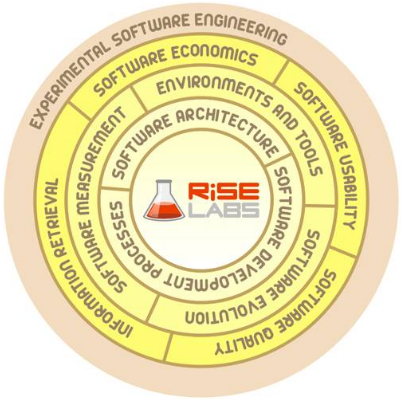
\includegraphics[width=9cm]{chapters/introduction/rise-spiral.png}
  \caption[RiSE Labs Influences]{RiSE Labs Influences}
  \label{fg:rise-spiral}
\end{center}
\end{figure}

Based on these areas, the RiSE Labs is divided in several projects, as shown in
Figure \ref{fg:rise-projects}. As it can be seen, this framework embraces
several different projects related to software reuse and software engineering.
They are:

\begin{itemize}
  \item \textbf{RiSE Framework:} Involves reuse processes
  \citep{Almeida2004,Nascimento2008}, component certification
  \citep{Alvaro2006} and reuse adoption process \citep{Garcia2008a}.
  
   \item \textbf{RiSE Tools:} Research focused on software reuse tools, such
   as the Admire Environment \citep{Mascena2006}, the Basic Asset Retrieval
   Tool (B.A.R.T) \citep{Santos2006}, which was enhanced with folksonomy
   mechanisms \citep{Vanderlei2007}, semantic layer \citep{Durao2008},
   facets \citep{Mendes2008} and data mining \citep{Martins2008}, and the
   Legacy InFormation retrieval Tool (LIFT) \citep{Brito2007}, the
   Reuse Repository System (CORE) \citep{CoreICSR}, and the Tool for Domain
   Analysis (ToolDAy) \citep{lisboa:msc:2008}. This dissertation is part of the RiSE tools;
   
   \item \textbf{RiPLE:}  Stands for RiSE Product Line Engineering Process and aims at developing   a methodology for Software Product Lines, composed of scoping \citep{Moraes2010},   requirements engineering \citep{neiva:msc:2009}, design \citep{filho:msc:2010,Cavalcanti:2011:ERP:2000259.2000286} , implementation, test \citep{neto:msc:2010,machado:msc:2010}, and evolution  management \citep{oliveira2009}.
   
   
   
   \item \textbf{SOPLE:} Development of a methodology for Service-Oriented Product Lines, based on the fundamentals of the RiPLE \citep{ribeiro2010}. 
   
   
   \item \textbf{MATRIX:} Investigates the area of measurement in reuse and
   its impact on quality and productivity;
   
   \item \textbf{BTT:} Research focused on tools for detection of duplicate
   bug reports, such as in \citet{CavalcantiFISL2008,CavalcantiInTech2012}.
   
   \item \textbf{Exploratory Research:} Investigates new research directions
   in software engineering and its impact on reuse;

   \item \textbf{CX-Ray:} Focused on understanding the \ac{C.E.S.A.R.}, and its
   processes and practices in software development.
\end{itemize}

This dissertation is part of the \ac{RiSE} Tools project. It was conducted in collaboration with researchers in software reuse , to solve the problem of traceability during the life-cycle of a\acf{SPL} development.


\begin{figure}[htp]
\begin{center}
  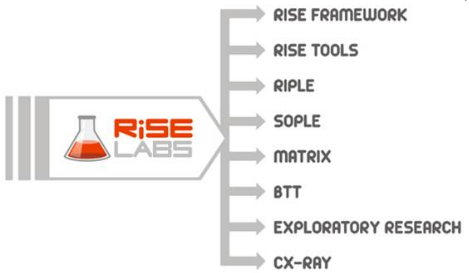
\includegraphics[width=10cm]{chapters/introduction/rise-projects.png}
  \caption[RiSE Labs Projects]{RiSE Labs Projects}
  \label{fg:rise-projects}
\end{center}
\end{figure}

\subsection{Outline of the Proposal}
This work defines the requirements, design and implementation of a software product lines lifecycle management tool, providing traceability and variability management and supporting most of the SPL process activities such as scoping, requirements, architecture, testing, version control, evolution, management and agile practices. In order to address it, we propose a metamodel that covers the SPL lifecycle, and develop a solution that consists in a Web based, extensible SPL lifecycle management tool, implementing this metamodel.  

The tool must enable the engineers involved in the process, to automatize the assets creation and maintenance, while providing traceability and variability management between them, providing detailed reports and enable the engineers to easily navigate between the assets using the traceability links. It must also provide a basic infrastructure for development, and a centralized point for user management among different tools.


\section{Out of Scope}
\label{sc:outofscope}

\begin{itemize}
  \item \textbf{ Full Application Engineering Support } Application engineering is the process of software product line engineering in which the applications of the product line are built by reusing domain artifacts and exploiting the product line variability \citep{Pohl2005}. Although the SPLICE architecture is flexible enough for it, we still do not support code binding, and cannot perform automatic product derivation.  
  
    \item \textbf{Risk Management.} Our metamodel do not support risk management assets yet.
    
    
  \item \textbf{Type of users.} The subjects of this work are
  developers and testers who will develop the system or test it. It also applies for stakeholders with some software engineering background, who understand the impact of their changes. Thus, it is out of scope  to provide a tool that supports the following types of users: business experts and end-users.
\end{itemize}

\section{Statement of the Contributions}
\label{sc:contributions}
As a result of the work presented in this dissertation, the following
contributions can be highlighted:
\begin{itemize}
\item \textbf{A study on SPL lifecycle management tools}, which can provide the research and professional community an overview of the state-of-the-art tools in the field considering the literature and tools on the market.


\item \textbf{A metamodel for Software Product Lines tools} that cover the activities of a \ac{SPL} development with agile practices and represent the interactions among the assets of a \ac{SPL}, as a way to provide traceability and variability, based on the metamodel developed in the \ac{RiSE} Labs \citep{Cavalcanti:2011}


\item \textbf{An application lifecycle management system} to support the suggested \ac{SPL} metamodel. A web-based, collaborative tool which acts as a centralized location to user-management, provide an infrastructure and support for the \ac{SPL} lifecycle steps.

\end{itemize}



\section{Dissertation Structure}
\label{sc:structure}
The remainder of this dissertation is organized as follows:

\begin{itemize}
\item \textbf{ Chapter \ref{ch:background} } reviews the essential topics used throughout this work: Software Product Lines and \ac{CASE} tools. It also contains a comprehensive revision similar tools.

\item \textbf{ Chapter \ref{ch:splice} } describes the functional and non-functional requirements proposed for the \ac{SPLICE} tool as well as architecture, the set of frameworks,the SPL metamodel and technologies used during the \ac{SPLICE} implementation.

\item \textbf{ Chapter \ref{ch:caseStudy} } describes an academic case study conducted to evaluate the tool.

\item \textbf{ Chapter \ref{ch:conclusion} } provides the concluding remarks. It discusses our contributions, limitations, threats to validity,  and outline directions for future work.




\end{itemize}

